\subsection[Dominance based ranking]{\label{identificadorReferenciaCruzada}
Dominance based ranking}

\ \ The dominance-based approaches use the concept of dominance for fitness assignment, contrary to other approaches that use a scalarization function or treat the various objectives separately. The main advantage of dominance-based approaches is that they don't need the transformation of the MOP into a single-objective problem.

There are several fitness assignment procedures based on dominance that can guide the search towards the Pareto border. The NSGA-II algorithm uses dominance depth where the population of solutions is decomposed into several fronts [5]. The non-dominated solutions of the population receive rank 1 and form the first front $E_{1}$. The solutions that are not dominated except by solutions of $E_{1}$ receive rank 2 and they form the second front $E_{2}$. In a general way, a solution receives
the row k if it is only dominated by individuals of the population belonging to the unit $E_{1} \cup ... E_{k-1}$. Then, the depth of the solution corresponds to the depth of the front to which it belongs. Since a single value fitness (rank) is assigned to every solution in the population, any search component of a single- objective metaheuristic can be used to solve MOPs. The bene t of using a Pareto- based fitness assignment such as this, compared to scalar methods, is that it evaluates the quality of a solution in relation to the whole population. No absolute values are assigned to solutions. Dominance depth rank assignment is shown on Figure 1.
\begin{figure}[h!]
\begin{center}
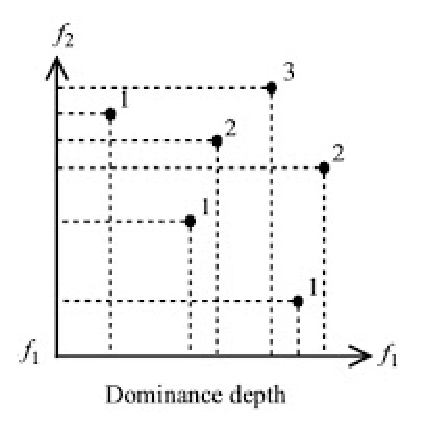
\includegraphics[width = 5cm] {./Graphics/Figure1.eps} 

\caption{Dominance depth [5]}
\end{center}
\end{figure}
